\documentclass[12pt]{article}
\usepackage[utf8]{inputenc}
\usepackage{amsmath}
\usepackage{graphicx}
\usepackage{float}
\title{MATLAB Model for Water Rocket Dynamics}
\author{Irving Rodriguez, Dan Sakaguchi, Eric Theis}
\date{}
\begin{document}
\begin{titlepage}
  \maketitle 
    \begin{abstract}
  A model was developed to accurately plot the height of a water rocket throughout its trajectory as a function of initial volume in the rocket at a given pressure, in our test cases, 40 psi. This model was created by simultaneously solving a set of four differential equations derived from Bernoulli's principles, an equation for adiabatic gas expansion, a quadratic air resistance model, and the rocket equation. The model was developed in Matlab and was then experimentally tested using a water rocket.
  \end{abstract}
\end{titlepage}
  \tableofcontents
  \pagebreak

  \section{Intro}
  Water rockets are used regularly in the classroom to demonstrate principles of momentum and its conservative properties. One of the many questions when using these rockets relates to how much water one should put in his or her rocket to maximize the height of its trajectory. The original purpose of our model was to provide a student building a bottle rocket the trajectory height maximizing volume of water to put in their rocket given a pressure. However, the granularity of data required to confirm our model over multiple pressures was less than our error. Based off this, we revised our model away from ideal volume given pressure towards predicting the height of the trajectory at a volume.
Initially, we hypothesized that the maximum height would be produced by the volume of water which would become completely expelled at the moment the pressures reach equilibrium.
  \section{Experiment}
  \subsection{Rocket Assembly}
For these experiments, we utilized the Pitsco Stratoblaster kit to construct our rocket. Three trapezoidal fins were hot glued every 3 inches around the 9” circumference of the 625mL bottle at the point of tapering. The 1” diameter air tube was hot glued to the bottom of the bottle. The cone of the rocket was glued to the bottle after sliding on the tube. Tape was placed all around the cone for waterproofing. The ping pong ball was then glued to the opposite end of the air tube. All glued surfaces were sanded down to create a flatter point of contact. 

\begin{figure}[H]
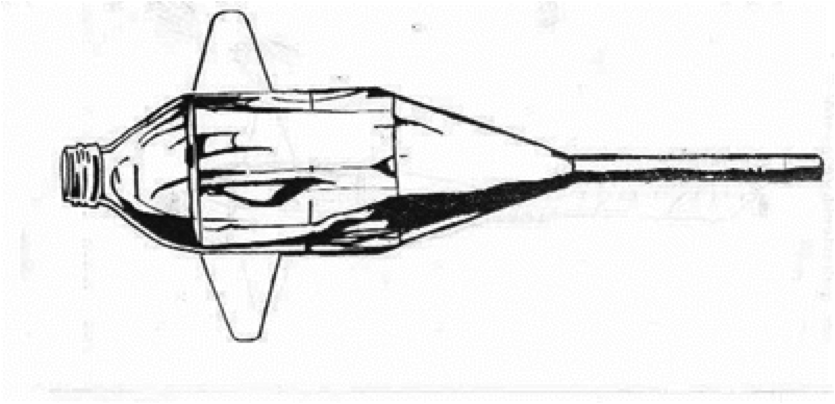
\includegraphics{rocketDiagram.png}
\centering
  \caption{Side view of final assembly of rocket. Fins are equally apart around  the circumference ($3^{rd}$ fin perpendicular to figure). Air tube is glued to bottle at opposite end of nozzle with cone attached. Ping pong ball (not shown) glued to end of air tube, opposite from cone.}
\end{figure}

These assembly instructions did not deviate from the kit instructions except regarding the use of a parachute. After test-launching the rocket both with a pre-manufactured plastic parachute and without, we qualitatively observed that the parachute does not provide a considerably slower descent after the rocket has reached its apogee. Using a parachute adds a sizable amount of time to each test run as it has to be reloaded after every launch. In addition, it is difficult to reload the parachute so that it deploys consistently. For these reasons, the fact that we planned to run a large amount of tests, the group member launching the rocket could simply catch it upon its return to the ground, and the rocket could be reassembled rather quickly if repairs were necessary, we decided to assemble our final rocket without a parachute. 

  \subsection{Materials}
Launches were performed using a tri-pod made of PVC pipe. A cylindrical top that fits flush with the nozzle of the bottle sits on the tripod in a chamber. The top is attached to a gas tube and is therefore semi-mobile; it can be detached from the chamber a few inches. This is important to launching since the bottle sits nozzle-down during launch. The only way to align the bottle in this way without losing any water inside the bottle is by detaching the top and inserting it into the nozzle . The gas tube is connected to a bike pump for pressurizing. The pressure gauge on the tri-pod was used during experiments as it was observed to realistically measure the pressure inside the bottle, as opposed to the bike pump’s gauge which showed rather erratic pressures at times.
    \subsection{Height Measurements}
    Height measurements were made in one plane with three group members. One member filled the bottle with the appropriate amount of water during each trial and launched the rocket. The second member remained sedentary 38 meters east of the launcher while the third did the same 44 meters west. The two recorders used angle guns to measure the angle from the horizontal to the rocket at its apogee, as demonstrated below.
    
\begin{figure}[H]
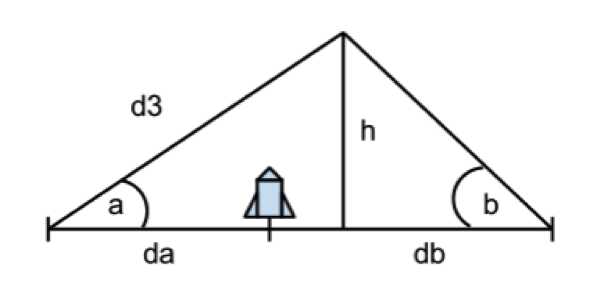
\includegraphics{heightDiagram.png}
\centering
  \caption{Two observers stand a distance da and db away from the launch point. Using    	angle guns, angles a and b are measured once the rocket has reached its max height h.}
\end{figure}

By measuring the height using this method, the rocket’s height can be calculated regardless of its horizontal displacement from the original launching point, assuming its trajectory remains in the plane of the two observers. By Law of Sines,

\begin{figure}[H]
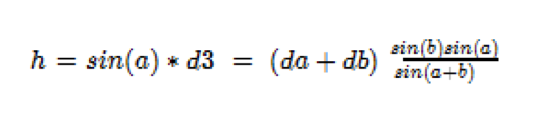
\includegraphics{trigEq2.png}
\centering
\end{figure}

The height of the trajectory can then be calculated:

\begin{figure}[H]
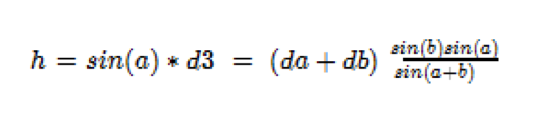
\includegraphics{trigEq2.png}
\centering
\end{figure}

    \subsection{Experiments}
    To find the maximum height of the trajectory, the volume of water in the rocket was varied from 0mL to 400mL in increments of 50mL. All launches were performed in as similar conditions as possible (~65 degrees celsius, 0-2mph winds) to reduce vairability in data from atmospheric conditions. 
A graduated cylinder was used to measure out the volume before each launch. Without the rocket attached, the bike pump was pumped 5 times prior to each launch to remove any leftover water in the gas tube from the previous launch. The rocket was then filled and the cylindrical top was placed inside the nozzle before being returned to the chamber. The holding apparatus was held in place by hand as the bottle was pumped until the system was pressurized so that it would not launch spontaneously on its own, held in place by the chamber. The launcher would then pump until the pressure gauge in the chamber stabilized at 40PSI. The rocket was then launched and the angles measured by the observers. This was performed 3 times for each increment of volume. The heights were calculated using Equation 2 and input into Microsoft Excel.
    The same procedure was used as in the first round of data collection, except the volumes ranged from 125mL to 225mL in increments of 25mL so as to properly deduce the true maximum of the data and ensure it did not lie in between increments of the previous experiment.
 \section{Physics and Model}
 \subsection{Setting up the Equations}
  % This is a comment; it is not shown in the final output.
  In creating a reasonable MATLAB model for the rocket dynamics, there are
  three relationships that must be considered
  \begin{enumerate}
  \item{Fluid dynamic relationship between internal pressure and 
  outward flow of fluid - given by Bernoulli's equation (for incompressible and compressible fluids)}
  \item{Dynamic relationship between exhaust velocity and acceleration of rocket - given by rocket equation}
  \item{Kinematic relationship between acceleration and position - given by basic kinematics}
\end{enumerate}
  
  We will now derive the relationships above. Most simply, we have for kinematic relationships,
  \begin{align}
    y\dot{} = v                             \\
    v\dot{} = y\ddot{} = a
  \end{align}
  
  Given a rocket with mass m, velocity v, exhaust velocity u, under the application of external force $F_{applied}$, we have the standard rocket equation,
  \begin{align}
  m\frac{dv}{dt}+u\frac{dm}{dt}=F_{applied}
  \end{align}
  
  With the only forces applied to the rocket being gravitational and from air drag, we have,
  \begin{align}
  F_{applied} = F_{gravity} + F_{drag} = -mg -\frac{1}{2}C_{d}\rho_{air}v^{2}
  \end{align}
  with $C_{d}$ the drag coefficient of the rocket. Assuming a coordinate system with $y\hat{}$ pointing up, $F_{drag}$ will point in the -$sign(v)y\hat{}$ direction, so 
  \begin{align}
  m\frac{dv}{dt}+u\frac{dm}{dt} = -mg - sign(v)\frac{1}{2}C_{d}\rho_{air}v^{2}
  \end{align}
  Now, we must consider the internal dynamics of water flow in the rocket. To avoid confusion, since a number of variables are used to derive these results, the following describes the meaning of each with their respective dimensions
  \begin{itemize}
  \item{$\rho_{air}$ - density of air ([$\frac{kg}{m^{3}}$])}
  \item{$\rho_{water}$ - density of water ([$\frac{kg}{m^{3}}$])}
  \item{$V_{air}$ - volume of air in rocket ([$m^{3}$])}
  \item{$V_{water}$ - volume of water in rocket ([$m^{3}$])}
  \item{$V_{tot}$ - total internal volume of rocket ([$m^{3}$])}
  \item{$A_{bottle}$ - area of bottle cross section ([$m^{2}$])}
  \item{$A_{nozzle}$ - area of bottle nozzle ([$m^{2}$])}
  \item{$P_{atm}$ - atmospheric pressure ([$\frac{kg}{ms^{2}}$])}
  \item{$P_{int}$ - internal pressure of rocket ([$\frac{kg}{ms^{2}}$])}
  \item{$\gamma$ - heat capacity ratio for air ([])}
  \item{$m_{rocket}$ - mass of rocket without water ([$kg$])}
  \end{itemize}
  
  First we note that since the density of water is constant, we have that $\frac{dm}{dt} = \rho_{water}\frac{dV_{water}}{dt} = \rho_{water}A_{nozzle}u$. So from (5)
  \begin{align}
  v\dot{}(m,m\dot{},v) = -\frac{1}{m\rho_{water}A_{nozzle}}m\dot{}^{2} -g - sign(v)\frac{1}{2m}C_{d}\rho_{air}v^{2}  
  \end{align}
  Between (2) and (6) now, it only remains to find $m\dot{}$ as a function of m, then we will have three differential equations which can be solved simultaneously by MATLAB. 
  
  In finding $\frac{dm}{dt}$, we consider two cases. 1) There is water and pressurized air in the bottle, with the exiting water consisting of the exhaust. 2) There is only pressurized air in the bottle, the exit of which then is the exhaust.
  
  \subsection{Case 1 - Incompressible Flow}
  In this case, we will use Bernoulli's principle in its standard form to relate internal variables with the outward rate of flow. Along a streamline from the top of the water column to the nozzle, Bernoulli gives
  \begin{align}
  \frac{v^{2}}{2} + gz + \frac{P}{\rho} = const
  \end{align}
  Since gravitation potential energies are negligible compared to kinetic, we will neglect the second term. At the top of the stream we have that $v_{top}=\frac{1}{A_{bottle}}\frac{dV_{air}}{dt}$ and at the bottom $v_{bottom}=\frac{1}{A_{nozzle}}\frac{dV_{air}}{dt}$, by continuity. Lastly, we make the assumption that the expansion in the bottle is rapid enough to be considered adiabatic. For an ideal gas undergoing adiabatic expansion, $PV^{\gamma} = const = P_{0}V_{0}^{\gamma}$, where $P_{0}, V_{0}$ are the initial pressure and volume, resp. So
  \begin{align}
  (\frac{1}{A_{bottle}})^{2}(\frac{dV_{air}}{dt})^{2} + \frac{2P_{0}V_{0}^{\gamma}}{V_{air}^{\gamma}\rho} = (\frac{1}{A_{nozzle}})^{2}(\frac{dV_{air}}{dt})^{2} + \frac{2P_{atm}}{\rho}
  \end{align}
  Solving for $\frac{dV_{air}}{dt}$ we have
  \begin{align}
  \frac{dV_{air}}{dt} = \frac{1}{\sqrt{(\frac{1}{A_{nozzle}})^{2} - (\frac{1}{A_{bottle}})^{2}}}\sqrt{\frac{2}{\rho}(\frac{P_{0}V_{0}^{\gamma}}{V_{air}^{\gamma}} - P_{atm})}
  \end{align}
  In order to relate this to m instead of V, we note that $\frac{dm}{dt} = \rho_{water}\frac{dV_{air}}{dt}$ and $m = m_{rocket} + \rho_{water}(V_{tot} - V_{air})$. So
  \begin{align}
  m\dot{}(m) = \frac{\rho_{water}}{\sqrt{(\frac{1}{A_{nozzle}})^{2} - (\frac{1}{A_{bottle}})^{2}}}\sqrt{\frac{2}{\rho}(\frac{P_{0}V_{0}^{\gamma}}{(V_{tot} - \frac{(m - m_{rocket})}{\rho_{water}})^{\gamma}} - P_{atm})}
  \end{align}  
  \subsection{Case 2 - Compressible Flow}
  Here we use Bernoulli's principle for compressible flow. For a streamline of air, by Bernoulli we have
  \begin{align}
  \frac{v^{2}}{2} + gz + (\frac{\gamma}{\gamma-1})\frac{P}{\rho} = const
  \end{align}
  By considering a streamline from the top of the bottom to the nozzle, ignoring the negligible gravity term, we have
  \begin{align}
  \frac{v^{2}}{2} + (\frac{\gamma}{\gamma-1})\frac{P_{atm}}{\rho} = (\frac{\gamma}{\gamma-1})\frac{P}{\rho}
  \end{align}  
  Since volume is fixed, yet the amount of gas changes, we have that $P = P_{i}\frac{m-m_{rocket}}{m_{0}-m_{rocket}}$ and $\rho = \rho_{0}\frac{m-m_{rocket}}{m_{0}-m_{rocket}}$. Also, we have that $P_{i} = \frac{P_{0}V_{0}^{\gamma}}{V_{tot}^{\gamma}}$. So
  \begin{align}
  v = \sqrt{(2\frac{\gamma}{\gamma-1})(\frac{m-m_{rocket}}{m_{0}-m_{rocket}}\rho_{0})(\frac{P_{0}V_{0}^{\gamma}}{V_{tot}^{\gamma}}\frac{m-m_{rocket}}{m_{0}-m_{rocket}} - P_{atm})}
  \end{align} 
  and 
    \begin{align}
    m\dot{}(m) = \rho_{air}A_{nozzle}\sqrt{(2\frac{\gamma}{\gamma-1})(\frac{m-m_{rocket}}{m_{0}-m_{rocket}}\rho_{0})(\frac{P_{0}V_{0}^{\gamma}}{V_{tot}^{\gamma}}\frac{m-m_{rocket}}{m_{0}-m_{rocket}} - P_{atm})}
  \end{align} 
  Now we have three differential equations which can be solved simultaneously.
  \begin{enumerate}
  \item{$m\dot{}(m)$ (piecewise defined depending on whether there is water left in the rocket)}
  \item{$v\dot{}(m,m\dot{},v$}
  \item{$y\dot{}(v)$}
  \end{enumerate}
  Here we have three differential equations that can be solved simultaneously using MATLAB's ode45() function. Unfortunately, the compressible Bernoulli model was unable to be developed thoroughly enough to give credible results, which we will discuss further in the analysis.
  \section{Code}
  \begin{verbatim}
File - rocketSolver.m
function [xprime] = rocket_solver2(t,x,V0,P0)
%% Meaning of x and xprime
% x(1) - amount of water in rocket
%       xprime(1) - velocity of water discharge
% x(2) - velocity of the rocket
%       xprime(2) - acceleration of the rocket
% x(3) - mass of the rocket
%       xprime(3) - rate of mass discharge
% x(4) - position of the rocket
%       xprime(4) - velocity of the rocket

%% define all constants used
rho = 1000;             %% kg/m^3
rho_air = 1.23;         %% kg/m^3
cd = .5;                %% []
B = .0014;              %% m^2
A = .00038;              %% m^2
Patm = 101350;          %% kg/(m*s)
g = 9.8;                %% m/s^2
Vtot = .625;               %% L

%%%%%%%%%%%%%%%%%%%%%%%%%%%%%%%%%%%%%%%%%%%%%%%%%%%

C = (P0*6900)*V0/1000; %% calc constant for gas pressures
D = 1 / sqrt(1/A^2 - 1/B^2); %% calc constant for dVa/dt
arg = (2/rho)*(C/x(1)-Patm); %% find argument of the sqrt function

%If all the water has been expelled or the pressures have equalized,
%then set dVa/dt to 0
if arg > .000001 && x(1) < Vtot/1000
    xprime(1,1) = D*sqrt(arg);
else
    xprime(1,1) = 0;
end

% Calculate the drag force using the current velocity

dragForce = cd / 2 * rho_air * B * x(2)^2;
xprime(2,1) = rho / (A*x(3)) * xprime(1,1)^2 - g - ...
sign(x(2)) * dragForce / x(3);
xprime(3,1) = - rho * xprime(1,1);
xprime(4,1) = x(2);
end

\end{verbatim}
\begin{verbatim}
  File - findTrajectory.m
  
function maxHeight = findTrajectory(waterAdded,P0,toPlot) 
% waterAdded in mL
m0 = .0575; % kg
rho_water = 1000; % kg/m^3
rho_air = 1.23; % kg/m^3    
Vtot = .000625;
m = m0 + rho_water * waterAdded/10^6 + rho_air * (P0/(101350/6900)) ...
* (Vtot - waterAdded/10^6);

V0 = Vtot - waterAdded/10^6;
[t y] = ode45(@(t,y)rocket_solver(t,y,V0,P0),0:5,[m 0 0]);
if toPlot
    figure('Name',['Theoretical Rocket Data for ', ...
    num2str(waterAdded),' ml of water']);
    subplot(2,2,1);
    plot(t,y(:,1));

    title('Mass (L) v. time (s)');
    subplot(2,2,2);
    plot(t,y(:,2));
    title('Velocity (m/s) v. time (s)');
    subplot(2,2,3);
    plot(t,y(:,3));
    title('Height (m) v. time (s)');
end
maxHeight = max(y(:,3));
end
    \end{verbatim}
  \section{Data and Analysis}
  \subsection{Analysis Methods}
  In order to compare the observed data and the model-predicted set, we computed error bars on the height measurements to see whether the model fit within these limits. 
  
  Assuming a constant $\sigma_{\theta} = 3^{\circ}$, we then used the equations
  \begin{align}
  \sigma_{h} = \frac{\partial h}{\partial \theta}\sigma_{\theta} \\
  w_{i} = \frac{1}{\sigma_{i}^{2}} \\
  x_{weighted} = \frac{\sum x_{i}w_{i}}{\sum w_{i}} \\
  \sigma_{weighted} = \frac{1}{\sum w_{i}}, i  \in \left\{1,2,3\right\}
  \end{align}
  
  to find the weighted error in our measurement.
  \subsection{Results}
The following figures graphically display the results of our data collection:

\begin{figure}[H]
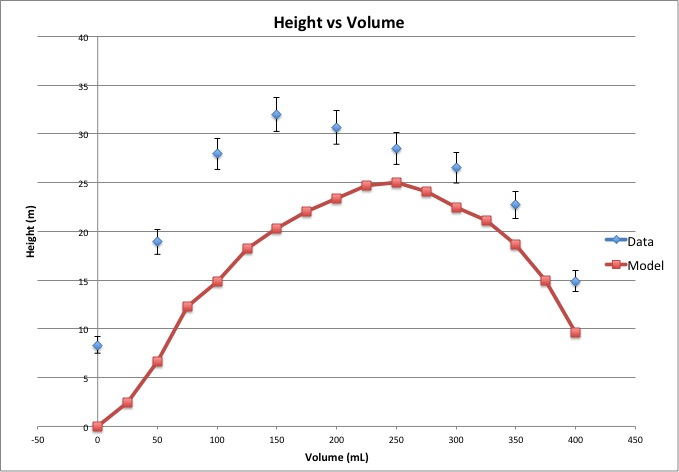
\includegraphics[scale=.5]{increment50mL.jpg}
\centering
\caption{Height vs. Volume at Volume Increments of 50 mL between 0 mL and 400 mL}
\end{figure}
    
\begin{figure}[H]
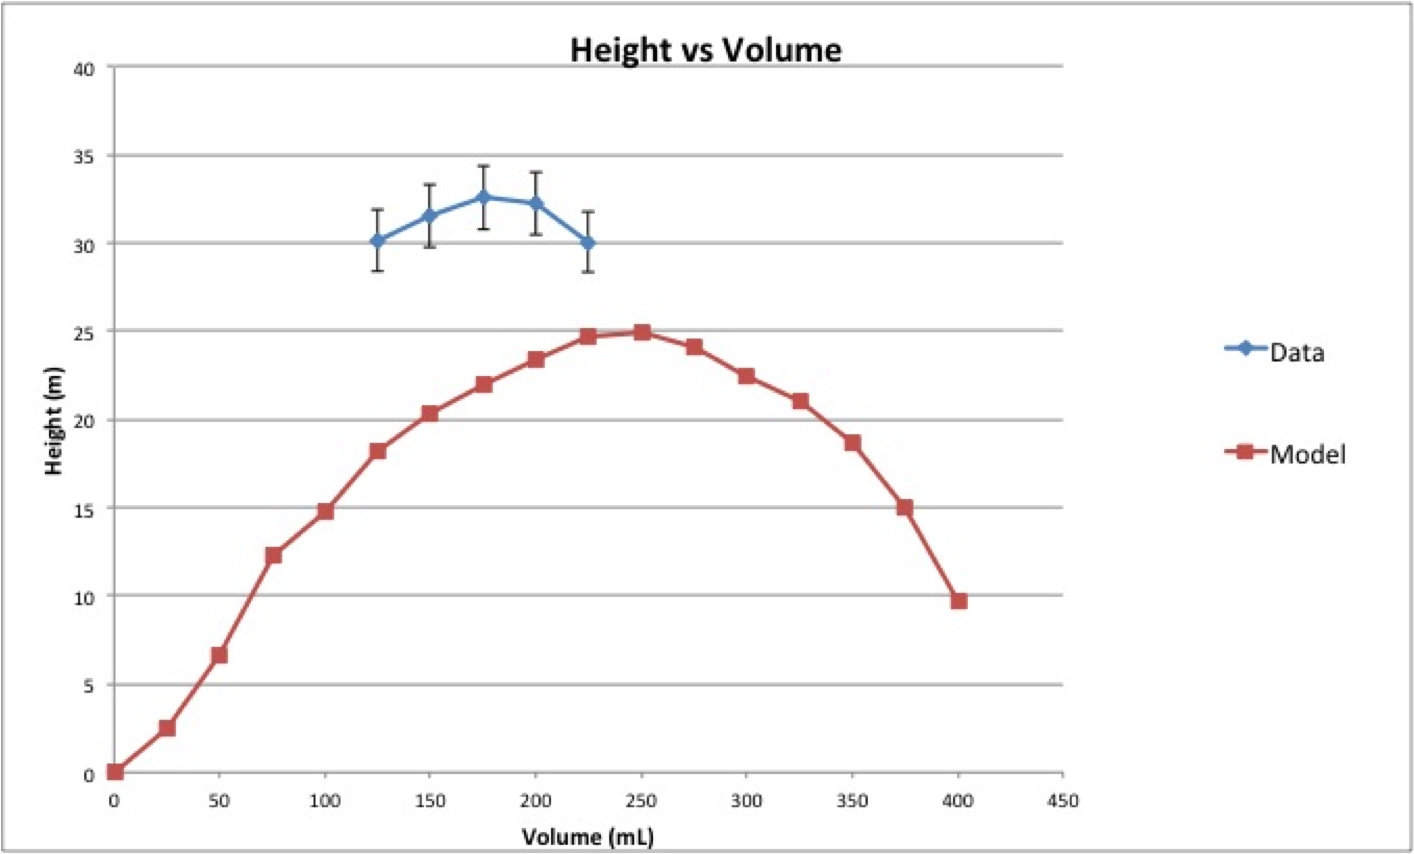
\includegraphics[scale=.5]{newdata.png}
\centering
\caption{Height vs. Volume at Volume Increments of 25 mL between 125 mL and 225 mL}
\end{figure}
  
  \subsection{Discussion}
  Overall, our model was somewhat accurate for volumes above 250 mL (within about 2 standard deviations), though it consistently projected heights about 4m below the measured heights. Below 250 mL, the model significantly varied from the measured results as seen below:
  
  \begin{figure}[H]
    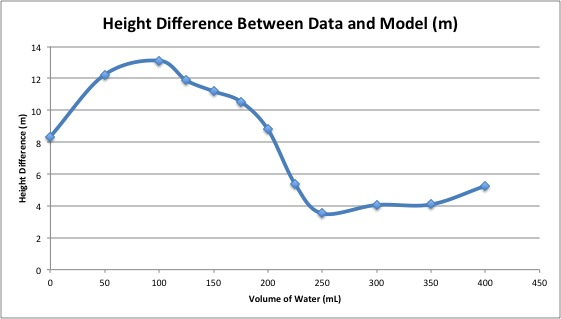
\includegraphics[scale=.5]{Difference.jpg}
    \centering
    \caption{difference between model and data at all measured volumes}
    \end{figure}
    
We made a variety of assumptions to create a model that was manageable to produce. The biggest of the assumptions we made was that air expelled from the rocket does not contribute to the force applied on the rocket. We think this is the reason our model diverged so greatly from the data at volumes below 250 mL, which appears to be the point at which there is just enough of a pressure differential to expel all the water, but not eject air (as shown by the large reduction in error above this volume). Additionally, it appears that our hypothesis that maximum height is produced below this “equilibrium” volume. We speculated that this is because the ratio of thrust provided to mass in the rocket isn’t actually maximized at the “equilibrium”, as air is significantly less dense than water.
  Another thing we assumed is that the way in which we applied Bernoulli's principles does not produce conservation of momentum of the water in the rocket after the pressures have equalized. Throughout the flight, the pressure differential accelerates the water downwards relative to the rest of the rocket. If the pressure equalizes before the water is completely expelled, the remaining water should still have some downward velocity. However, Bernoulli’s equations indicated that when pressure is equalized, the velocity of the water relative to the rocket is also zero. Thus, we assumed the later is true. This likely contributes to the fact that our model projects lower heights than the data presents above 250 mL.
  We used equations assuming laminar and adiabatic flow in our model and also assumed that both the water and rocket are in the same inertial reference frame. We also assumed in our equations that the shape of the water’s discharge was cylindrical with the same radius as the orifice at the bottom of the bottle. The actual discharge shape is seen below:
  
  \begin{figure}[H]
    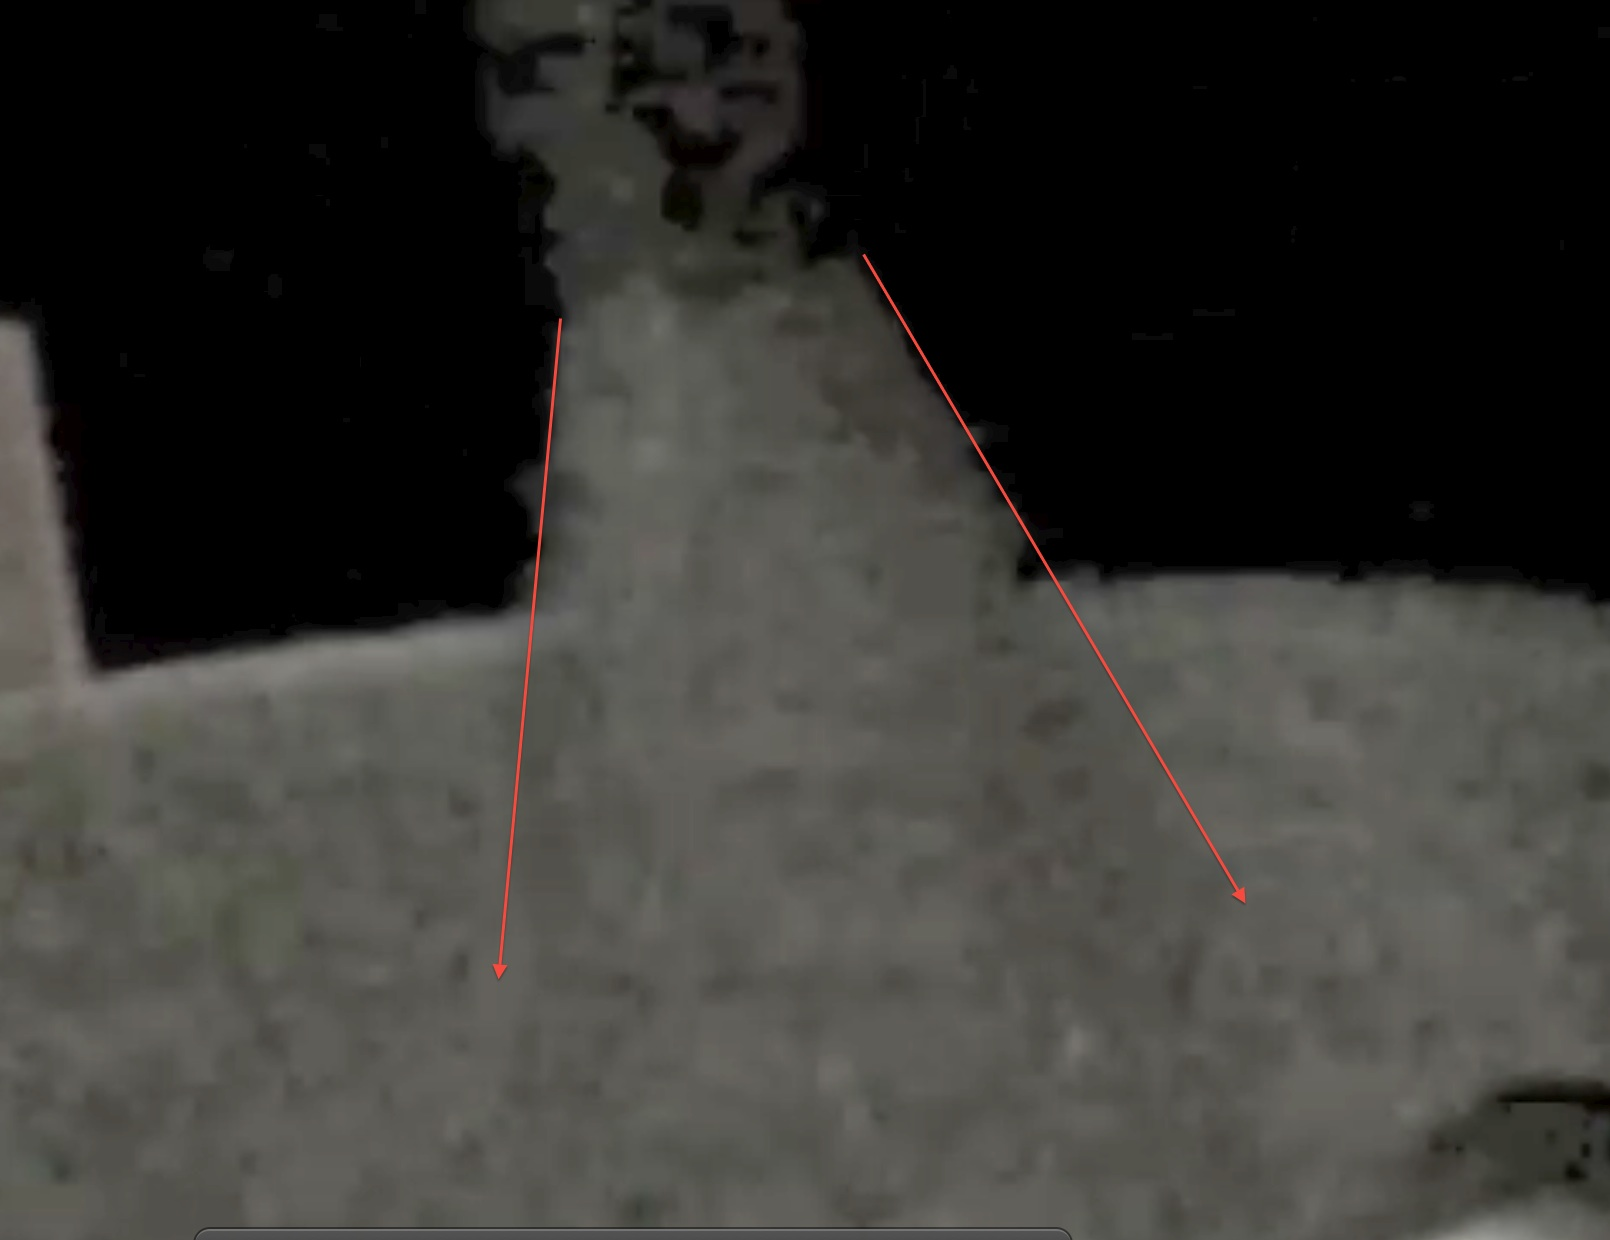
\includegraphics[scale=.3]{RocketCone.jpg}
    \centering
    \caption{The red arrows above indicate the edge of the discharge cone at the bottom of the rocket.}
    \end{figure}
  \subsection{Aside}
   The image below shows an attempt at modeling the correlation between volume and height while taking into account expulsion of air after all water has been discharged. Despite thoroughly checking the code (asside from going into the ode45 function), we were not able to eliminate the large, jagged variations in height for values below 250 mL, indicating that there is an issue with the way the expulsion of air is incorporated into the integration process. The interesting part of this image is that the peaks of the jagged graph form the same shape as the data we gathered and the minimums form the shape of our initial refined model.
  
    \begin{figure}[H]
    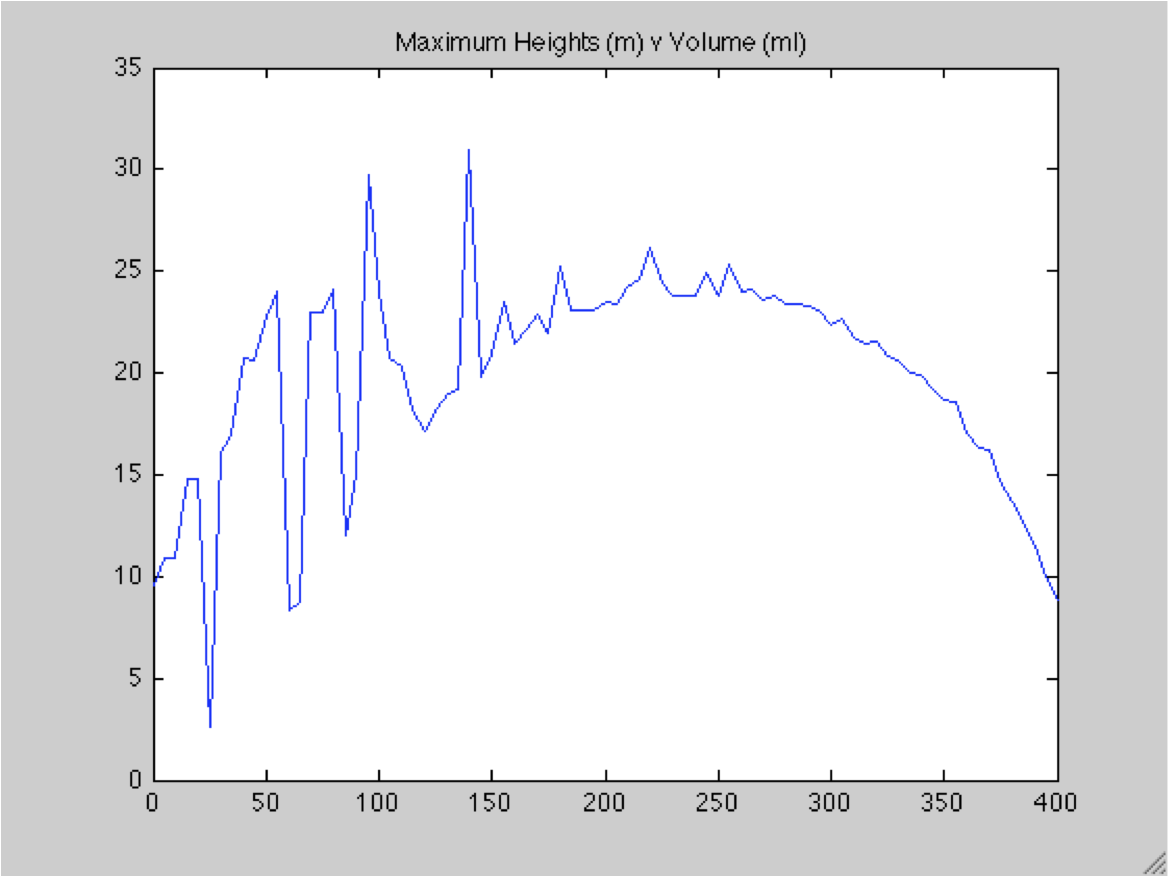
\includegraphics[scale=.3]{compressibleBernoulli.png}
    \centering
    \caption{Correlation between water in rocket and height accounting for explusion of air as well as water.}
    \end{figure}
  
  \section{Conclusion}
  
  Overall, our equations make too many assumptions to create an accurate model of maximum height. However, it is a good approximation of trajectory for volumes above what will be ejected by an equalizing pressure differential. In this domain, the projected height is lower than the measured height, but by a fairly consistent amount between datapoints (the shape of the curve is the same). In the future, it would be useful to finish expanding the model to include the thrust created due to air. Future work would also include testing the model at other pressures to confirm its reliability outside of 40 psi. After testing the model at different pressures, one could expand it to fulfill our original plan: a model of height maximizing volumes as a function of pressure.
  
  \section{Appendix}
  \subsection{Code for Compressible Bernoulli}
  \begin{verbatim}
  File - rocket_solver.m
  
function [xprime] = rocket_solver(t,x,V0,P0)
%% Meaning of x and xprime
% x(1) - mass inside the rocket
%       xprime(1) - rate of mass discharge
% x(2) - velocity of the rocket
%       xprime(2) - acceleration of the rocket
% x(3) - position of the rocket
%       xprime(3) - velocity of the rocket

%% Rename the x variables
mass = x(1);
velocity = x(2);

%% define all constants used
rho_water = 1000;      %% kg/m^3
rho_air = 1.23;         %% kg/m^3
drag_coeff = .5;         %% []
area_bottle = .0014;              %% m^2
area_nozzle = .00038;              %% m^2
pressure_atm = 101350;          %% kg/(m*s)
g = 9.8;                %% m/s^2
volume_total = .625/10^3;               %% m^3
mass_rocket = .0575; % kg
gamma = 7/5;
air_constant = gamma/(gamma - 1);

%%%%%%%%%%%%%%%%%%%%%%%%%%%%%%%%%%%%%%%%%%%%%%%%%%%

% Calculate volume of water in the bottle - ignore air-mass
% contribution, since it's negligible in this calculation
mass_internal = mass - mass_rocket;
waterVolume = mass_internal / rho_water;
airVolume = volume_total - waterVolume;

C = (P0*6900)*V0; %% calc constant for gas pressures
% Calculate the pressure the bottle would be under when the water has
% all left
pressure_emptyBottle = C/volume_total; 
% Calculate the density of the air would be when the water has all left
mass_emptyBottle = volume_total*rho_air* ...
(pressure_emptyBottle/pressure_atm);

massRate = 0;

% Calculate the drag force using the current velocity

dragForce = .5 * drag_coeff * rho_air * area_bottle * velocity^2;

% As soon as just enough mass for a bottle containing air at the 
%pressure for which V = volume_total, switch to
% compressible Bernoullli model
if mass_internal > mass_emptyBottle
    % Calculations with incompressible Bernoulli 
    
    D = 1 / sqrt(1/area_nozzle^2 - 1/area_bottle^2); 
    %% calc constant for dVa/dt
    arg = (2/rho_water)*(C/airVolume-pressure_atm); 
    %% find argument of the sqrt function

    % Assume that once the pressures have equalized inside the
    % container, the water mass has 0 velocity
    if arg > 0
        massRate = -D*sqrt(arg)*rho_water;
    else
        massRate = 0;
    end
    
    acceleration = massRate * (massRate / (area_nozzle*rho_water*mass))  ...
    - g - sign(velocity) * dragForce / mass;
else
    % Calculations with compressible Bernoulli
    
    % Calculate current pressure of bottle, now with constant volume
    % instead of mass
    pressure_internal = pressure_emptyBottle * ...
    (mass_internal / mass_emptyBottle);
    
    if pressure_internal < pressure_atm
        % the rocket's really empty now. You're done
        massRate = 0;
    else
        E = air_constant / rho_air;
        massRate = -rho_air * area_nozzle * sqrt(2*E* ...
        (pressure_internal - pressure_atm));
    end
    
    acceleration = massRate * (massRate / (area_nozzle*rho_air*mass))  ...
    - g - sign(velocity) * dragForce / mass;

end
    xprime(1,1) = massRate;
    xprime(2,1) = acceleration;
    xprime(3,1) = velocity;
end
  \end{verbatim}
  
  \subsection{Analysis of Height Measurement Technique}
\end{document}